\documentclass{article}

\usepackage[dvipsnames]{xcolor}
\usepackage{tikz}
\usepackage{listings}

\title{Software Saturdays Quiz 1}
\author{Ryan Baker}
\date{\today}

\definecolor{JadeGreen}{RGB}{91,158,62}
\lstdefinestyle{catppuccin}{
	backgroundcolor=\color{White},
	commentstyle=\color{Gray},
	numberstyle=\footnotesize\ttfamily\color{Gray},
	stringstyle=\color{JadeGreen},
	keywordstyle=\color{BurntOrange},
	basicstyle=\ttfamily\footnotesize\color{Black},
	breakatwhitespace=false,
	breaklines=true,
	captionpos=b,
	keepspaces=true,
	numbers=left,
	numbersep=5pt,
	showspaces=false,
	showstringspaces=false,
	showtabs=false,
	tabsize=4
}
\lstset{style=catppuccin}

\begin{document}

\maketitle

\subsection*{Instructions}

\noindent
This quiz contains 8 questions. Submit your answers to each question to Brightspace. You are encourages to run code segments on your machine if you are stuck.

\subsection*{Quiz}

\begin{enumerate}

\item Which of the following is the purpose of the \texttt{main()} function?

\begin{itemize}
	\item[(a)] Declares global variables to be used by all files in the project
	\item[(b)] Serves as the entry point where program execution begins
	\item[(c)] It controls the flow of the compilation and linking process
	\item[(d)] The function \texttt{main()} has no special purpose, it can have any name
\end{itemize}

\item Match each stage of the C++ build process with its output file type:

\begin{center}
{
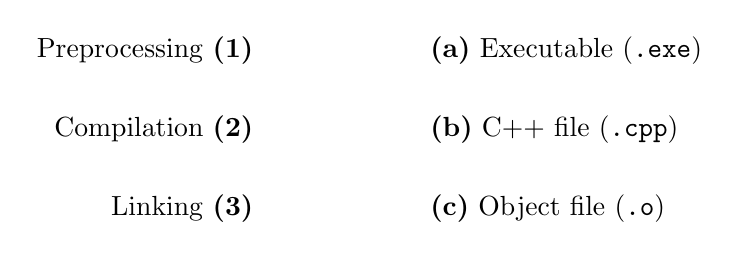
\begin{tikzpicture}
	\draw
	(0,2) node[left]  {Preprocessing \textbf{(1)}}
	(0,1) node[left]  {Compilation \textbf{(2)}}
	(0,0) node[left]  {Linking \textbf{(3)}}
	(2,2) node[right] {\textbf{(a)} Executable (\texttt{.exe})}
	(2,1) node[right] {\textbf{(b)} C++ file (\texttt{.cpp})}
	(2,0) node[right] {\textbf{(c)} Object file (\texttt{.o})}
	;
\end{tikzpicture}
}
\end{center}

\item Which of the following accurately describes a ``translation unit''?

\begin{itemize}
	\item[(a)] A \texttt{.cpp} file, plus the content of any files \texttt{\#include}'d
	\item[(b)] A single object file output by the compiler
	\item[(c)] A chunk of code that the compiler translates into machine code
	\item[(d)] The final executable file after the linking process
\end{itemize}

\item Which does the preprocessor \textbf{NOT} do in the C++ build process?
\begin{itemize}
	\item[(a)] Performs text replacement using {\texttt{\#define}}
	\item[(b)] Copies and pastes files using {\texttt{\#include}}
	\item[(c)] Conditionally compiles code with {\texttt{\#if}}, {\texttt{\#ifdef}}, and {\texttt{\#ifndef}}
	\item[(d)] {Translates C++ code into machine code}
\end{itemize}

\item What is the output of the following code:
\lstinputlisting[language=C++]{sizeof.cpp}
\begin{itemize}
	\item[(a)] \texttt{1, 2, 3, 4}
	\item[(b)] {\texttt{1, 2, 4, 8}}
	\item[(c)] \texttt{2, 4, 8, 16}
	\item[(d)] \texttt{8, 16, 32, 64} 
\end{itemize}

\item What is the output of the following code:

\lstinputlisting[language=C++]{main.hpp}
\lstinputlisting[language=C++]{openbrace.txt}
\lstinputlisting[language=C++]{closebrace.txt}
\lstinputlisting[language=C++]{helloworld.cpp}

\begin{itemize}
	\item[(a)] Hello, World!
	\item[(b)] Compilation error
	\item[(b)] Linking error
	\item[(c)] Runtime error 
\end{itemize}

\pagebreak

\item You attempt to build your C++ project with your favorite compiler and see the following message:

\lstinputlisting[]{lderror.txt}

\noindent
Which type of error is this?

\begin{itemize}
	\item[(a)] Compilation error
	\item[(b)] {Linking error}
	\item[(c)] Runtime error
\end{itemize}

\item Which of the following is true about C++'s builtin datatypes?

\begin{itemize}
	\item[(a)] The \texttt{int} type is guaranteed to occupy 4 bytes
	\item[(b)] The only real difference between datatypes is their size (\texttt{sizeof})
	\item[(c)] The \texttt{bool} type represents True and False, and occupies one bit
	\item[(d)] \texttt{sizeof(void)} is guaranteed to be greater than or equal to \texttt{sizeof(int)}
\end{itemize}

\end{enumerate}

\end{document}